Nous créons une fonction sinus avec les caractéristiques suivantes:\\
\begin{itemize}
\item Fréquence d'échantillonnage : 10 kHz
\item Fréquence du signal : 1 kHz 
\end{itemize}


\begin{figure}[H]
\centering
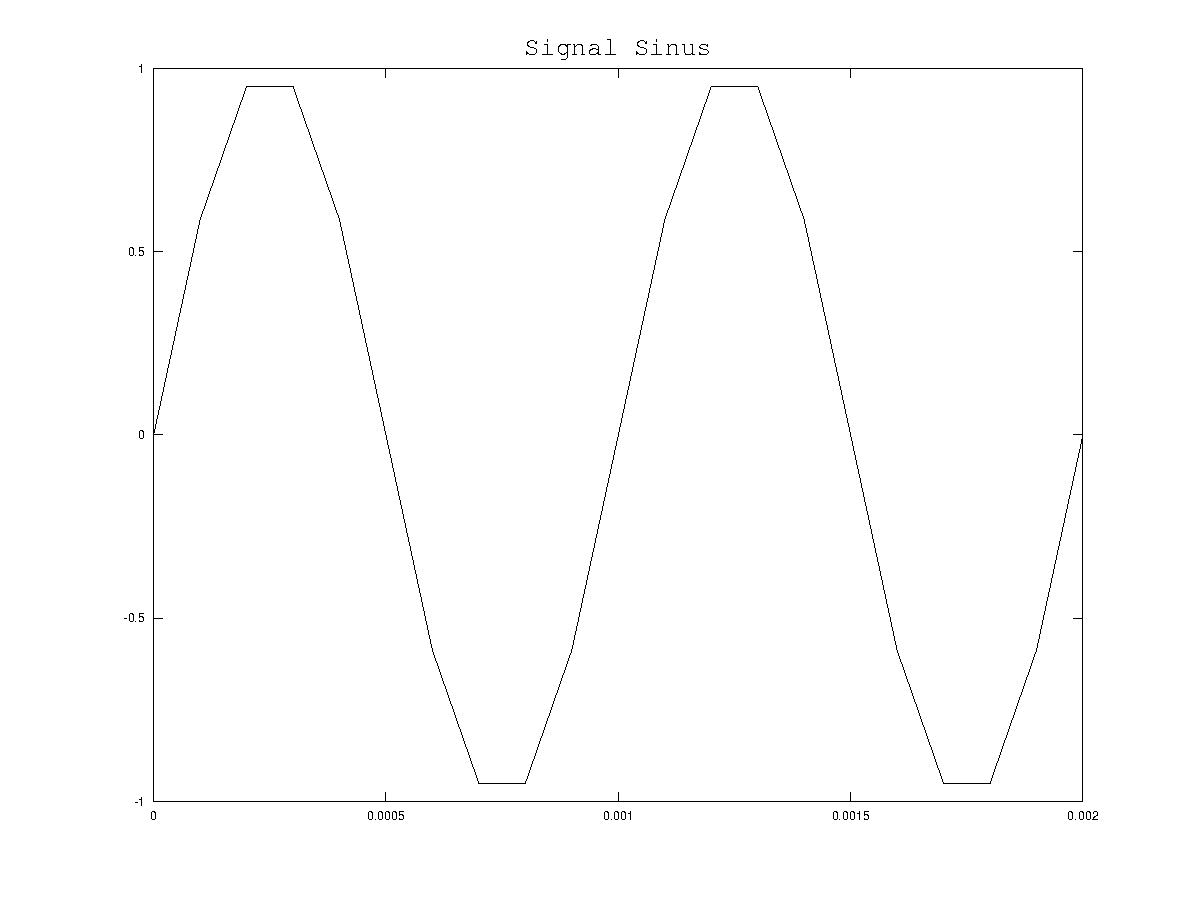
\includegraphics[width=9cm]{resEx5/fig_1_sinus.pdf}
\caption{Signal Sinus : x=$sin(2*pi*fsig*t)$}
\end{figure}


Nous ajoutons un bruit gaussien avec les caractéristiques suivantes:\\
\begin{itemize}
\item Moyenne : null
\item Amplitude : 0.4
\end{itemize}

\begin{figure}[H]
\centering
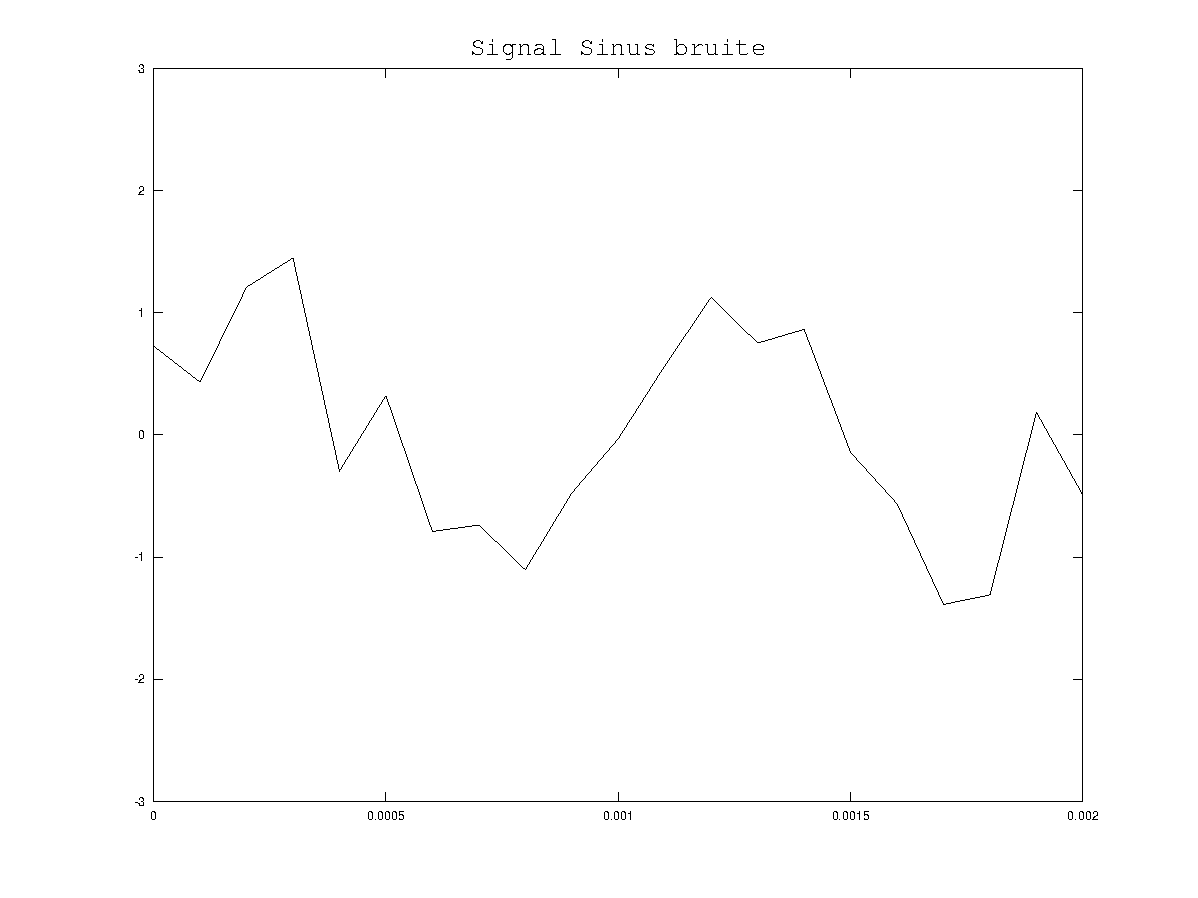
\includegraphics[width=9cm]{resEx5/fig_2_sinusb.pdf}
\caption{Signal Sinus bruité : xB=$ x .+ (moy + ampl*rand(1,N))$}
\end{figure}


Creation d'un filtre passe-bande avec buttord ayant les caractéristiques suivantes:\\
\begin{itemize}
\item Propriété : Ws(1) < Wp(1) < Wp(2) < Ws(2)
\item Ws(1) : 50 
\item Wp(1) : 980 
\item Wp(2) : 1020 
\item Ws(2) : 1450 
\end{itemize}


\begin{figure}[H]
\centering
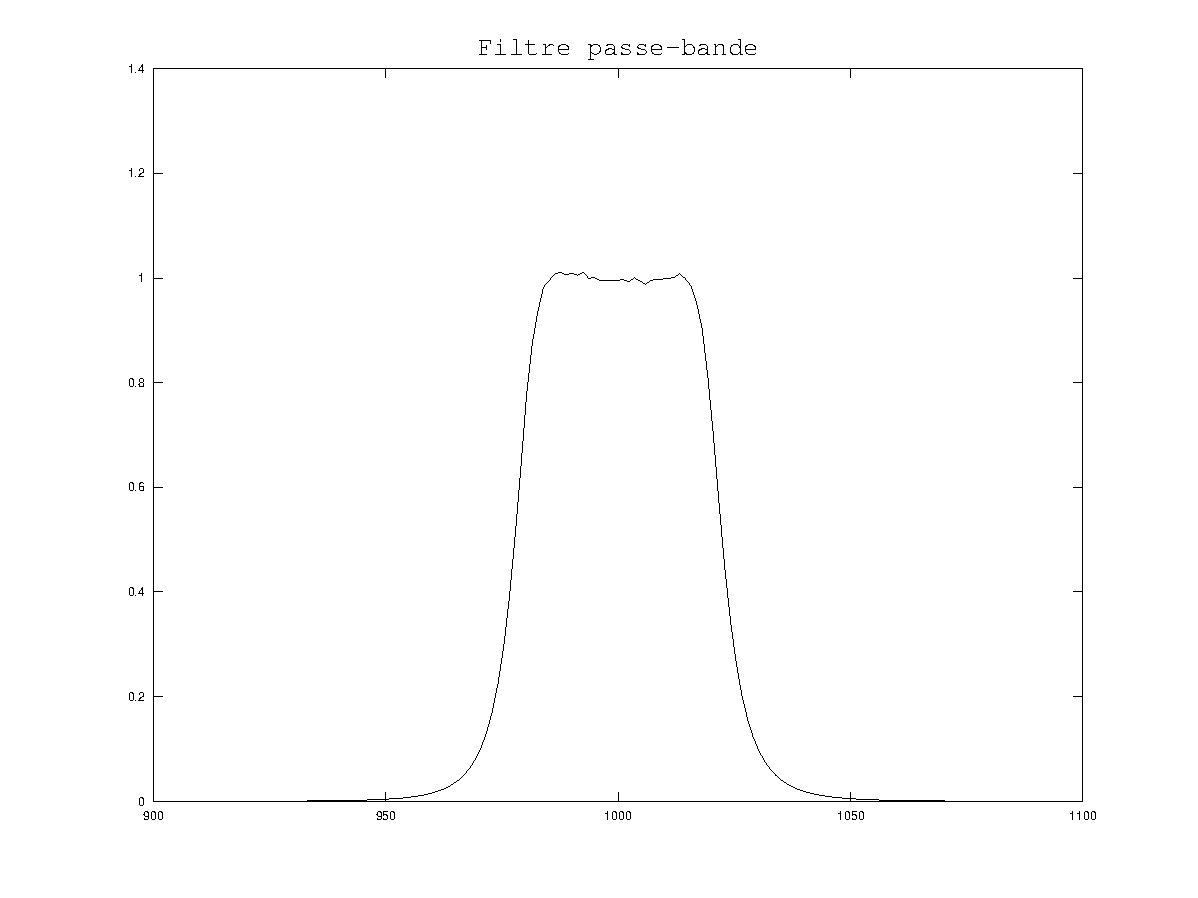
\includegraphics[width=9cm]{resEx5/fig_3_passbande.pdf}
\caption{Filtre Bande Passante visualisé sur l'intervale [900,1100]}
\end{figure}


\begin{figure}[H]
\centering
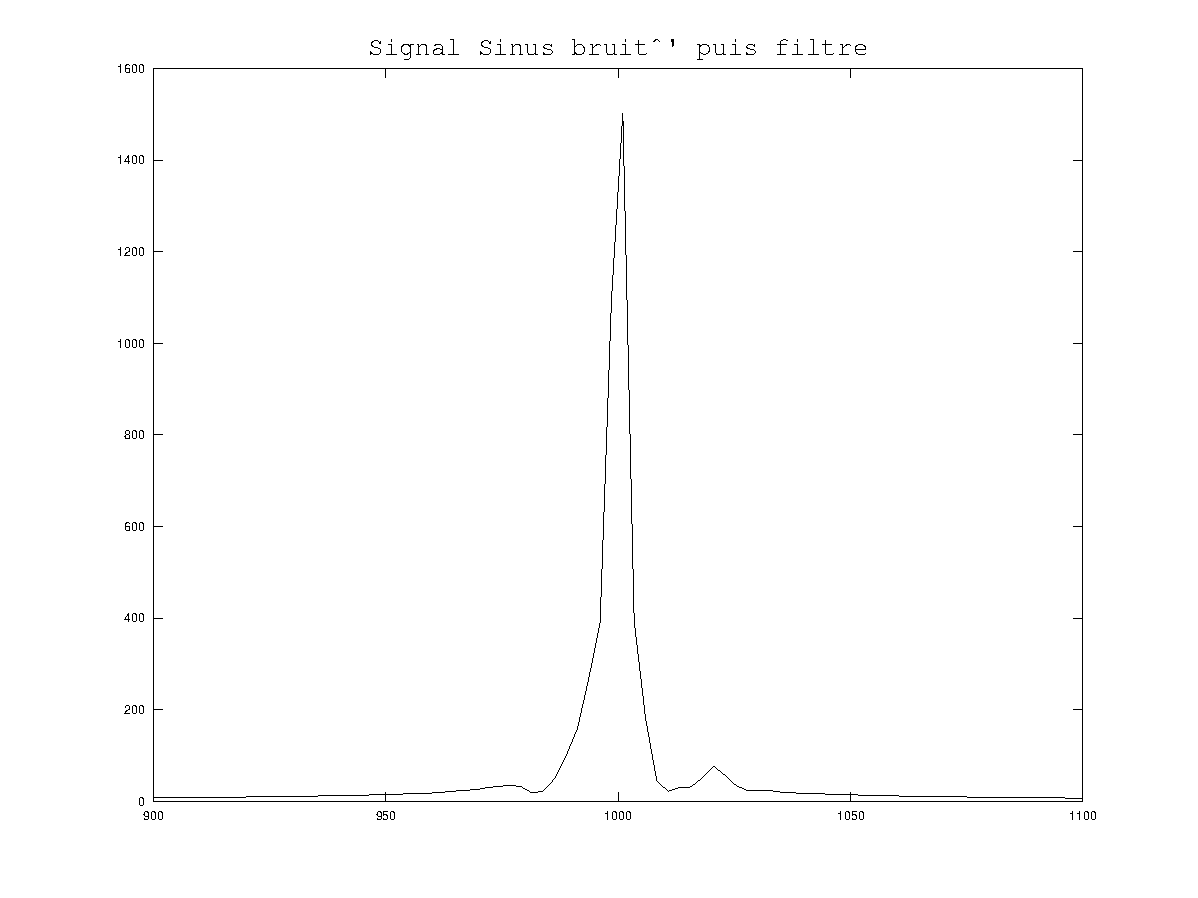
\includegraphics[width=9cm]{resEx5/fig_5_sinus-b.pdf}
\caption{Application du Filtre Bande Passante}
\end{figure}


\begin{figure}[H]
\centering
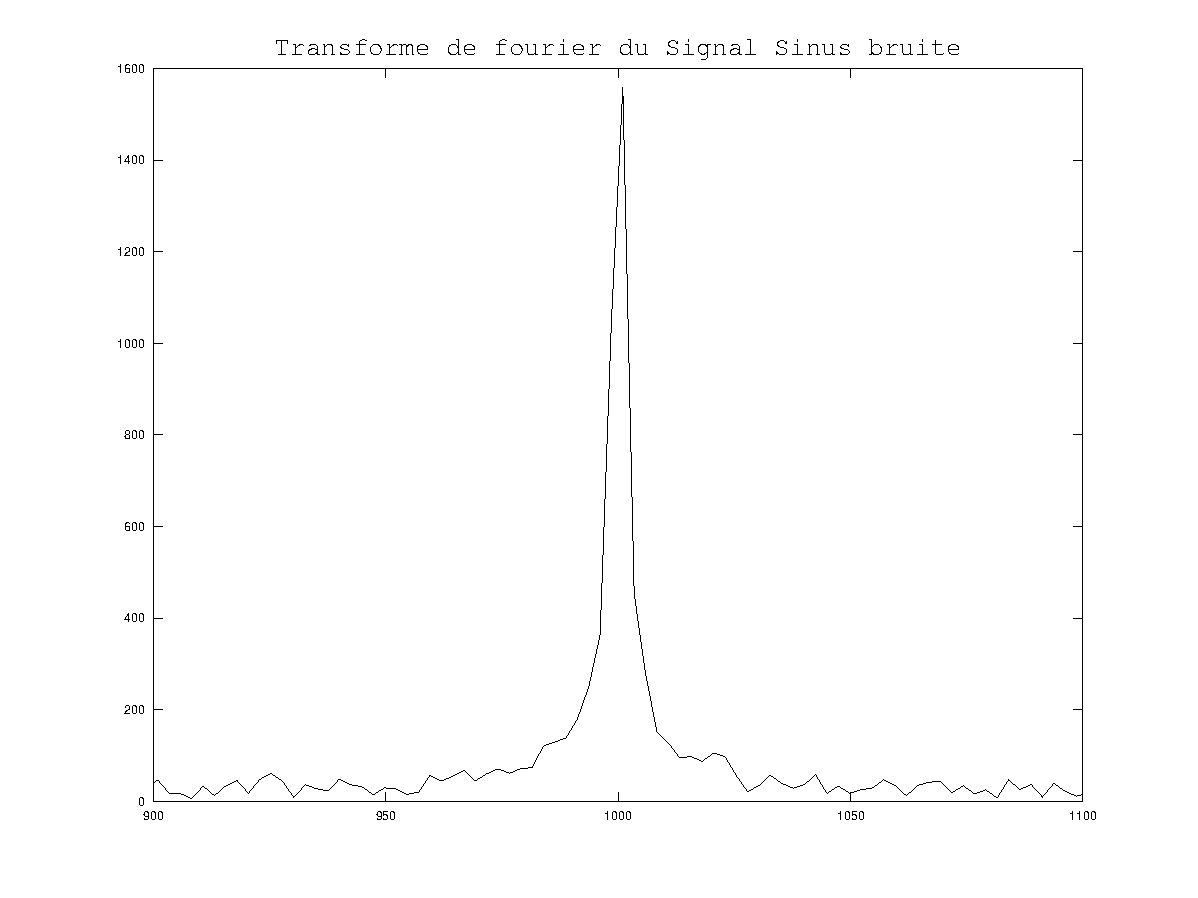
\includegraphics[width=9cm]{resEx5/fig_4_fftsinusb.pdf}
\caption{Transforme de fourier du Signal Sinus bruite}
\end{figure}


En comparant la courbe de la transformation de fourier du signal bruité FIG 42 et la courbe du signal bruité filtré FIG 41, nous remarquons autour de la frequence 1KHz ( le pic de la courbe ) que le bruit discorde moins la courbe et à donc été atténué .


